\documentclass[12pt]{article}
\usepackage{amsmath}
\usepackage{graphicx}
\usepackage{hyperref}
\usepackage{listings}
\usepackage{color}
\usepackage{pythonhighlight}
\usepackage{float}

\title{Operating System Course Report - First Half of the Semester}
\author{A class}
\date{\today}

\begin{document}

\maketitle
\newpage

\tableofcontents
\newpage

\section{Introduction}
This report summarizes the topics covered during the first half of the Operating System course. It includes theoretical concepts, practical implementations, and assignments. The course focuses on the fundamentals of operating systems, including system architecture, process management, CPU scheduling, and deadlock handling.

\section{Course Overview}
\subsection{Objectives}
The main objectives of this course are:
\begin{itemize}
    \item To understand the basic components and architecture of a computer system.
    \item To learn process management, scheduling, and inter-process communication.
    \item To explore file systems, input/output management, and virtualization.
    \item To study the prevention and handling of deadlocks in operating systems.
\end{itemize}

\subsection{Course Structure}
The course is divided into two halves. This report focuses on the first half, which covers:
\begin{itemize}
    \item Basic Concepts and Components of Computer Systems
    \item System Performance and Metrics
    \item System Architecture of Computer Systems
    \item Process Description and Control
    \item Scheduling Algorithms
    \item Process Creation and Termination
    \item Introduction to Threads
    \item File Systems
    \item Input and Output Management
    \item Deadlock Introduction and Prevention
    \item User Interface Management
    \item Virtualization in Operating Systems
\end{itemize}

\section{Topics Covered}

\subsection{Basic Concepts and Components of Computer Systems}
This section explains the fundamental components that make up a computer system, including the CPU, memory, storage, and input/output devices.

\subsection{System Performance and Metrics}
This section introduces various system performance metrics used to measure the efficiency of a computer system, including throughput, response time, and utilization.

\subsection{System Architecture of Computer Systems}
Describes the architecture of modern computer systems, focusing on the interaction between hardware and the operating system.

\subsection{Process Description and Control}
Processes are a central concept in operating systems. This section covers:
\begin{itemize}
    \item Process states and state transitions
    \item Process control block (PCB)
    \item Context switching
\end{itemize}

\subsection{Scheduling Algorithms}
This section covers:
\begin{itemize}
    \item First-Come, First-Served (FCFS)
    \item Shortest Job Next (SJN)
    \item Round Robin (RR)
\end{itemize}
It explains how these algorithms are used to allocate CPU time to processes.

\subsection{Process Creation and Termination}
Details how processes are created and terminated by the operating system, including:
\begin{itemize}
    \item Process spawning
    \item Process termination conditions
\end{itemize}

\subsection{Introduction to Threads}
This section introduces the concept of threads and their relation to processes, covering:
\begin{itemize}
    \item Single-threaded vs. multi-threaded processes
    \item Benefits of multithreading
\end{itemize}

\begin{figure}[h]
    \centering
    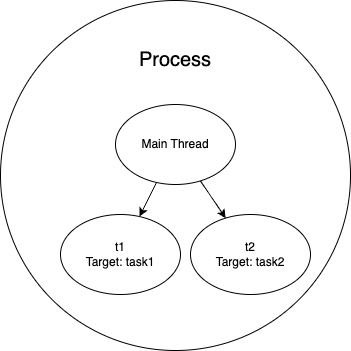
\includegraphics[width=0.5\textwidth]{/Users/khawaritzmi/Unhas/os_report_mid2024/a_class/asset/example.png}  % Sesuaikan nama file dan ukurannya
    \caption{Ini adalah gambar contoh dari multithreading.}
    \label{fig:contoh_gambar}
\end{figure}

Seperti yang terlihat pada Gambar \ref{fig:contoh_gambar}, inilah cara menambahkan gambar dengan keterangan.

\subsection{File Systems}
File systems provide a way for the operating system to store, retrieve, and manage data. This section explains:
\begin{itemize}
    \item File system structure
    \item File access methods
    \item Directory management
\end{itemize}

\subsection{Input and Output Management}
Input and output management is key for handling the interaction between the system and external devices. This section includes:
\subsubsection{Pengertian \textit{Input} dan \textit{Output}}
\textit{Input/Output} adalah suatu perangkat yang berhubungan dengan sistem komputer dengan cara mengirim sinyal melalui suatu kabel atau bahkan melalui udara .\\
\begin{enumerate}
    \item \textit{Input}.
    \textit{Input} adalah semua data dan perintah yang dimasukkan ke dalam memori komputer untuk diproses lebih lanjut oleh prosesor(Gallo, 2024).
    Contoh: data (angka, teks, gambar), perintah (klik \textit{mouse}, ketikan \textit{keyboard}, perintah suara).\\
    \item \textit{Output}.
    \textit{Output} adalah hasil dari pemrosesan data oleh komputer. Setelah menerima dan memproses \textit{input}, komputer menghasilkan \textit{output} yang bisa berupa informasi atau tindakan (Gallo, 2024).
    Contoh: hasil visual (tampilan di layar monitor), cetakan fisik (dokumen dari \textit{printer}), \textit{Audio} (notifikasi dari \textit{speaker}), \textit{file} (dokumen digital, \textit{spreadsheet}).\\
\end{enumerate}
\subsubsection{Konsep \textit{Input/Output}}
Alifiah dkk (2024) menjelaskan bahwa konsep \textit{input/output} secara umum ada tiga, yaitu:
\begin{enumerate}
    \item \textit{Port}. \textit{Port} ialah koneksi yang digunakan oleh perangkat untuk berkomunikasi dengan mesin. 
    \item \textit{Bus (Daisy Chain/ Shared Direct Access)}. \textit{Bus }ialah koneksi yang menghubungkan beberapa perangkat menggunakan kabel-kabel.
\begin{figure}[h]
\centering
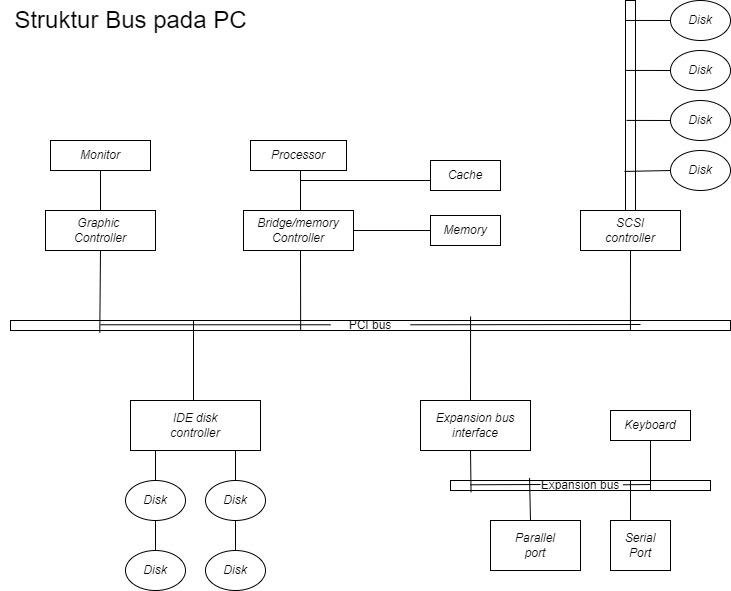
\includegraphics[width=0.5\textwidth]
{/asset/busPC.jpg}  % Sesuaikan nama file dan ukurannya
\caption{Struktur \textit{Bus} pada PC}
\label{fig:contoh_gambar}
\end{figure}
Struktur logika komputer pribadi memiliki sebuah \textit{bus} tunggal yang digunakan untuk menghubungkan CPU, memori, dan piranti-piranti I/O. Sebagian besar sistem memiliki dua \textit{bus} atau lebih (\textit{bus} kecepatan tinggi, untuk papan-papan I/O modern) dan bus kecepatan rendah (untuk papan-papan I/O yang lebih lama). Macam-macam Bus:
\begin{enumerate}
    \item \textit{Bus Arbiter} adalah sebuah \textit{chip} yang menentukan untuk mendapatkan giliran pertama penggunaan \textit{bus}.
    \item \textit{Bus} \textit{Industry Standard Architecture} (ISA) adalah suatu rancangan komputer yang tetap mempertahankan \textit{bus} PC lama.
    \item \textit{Bus} \textit{Extended} ISA (EISA ) adalah suatu rancangan komputer yang menggunakan \textit{multiple bus} dimana salah satu busnya adalah \textit{bus} ISA.
    \item \textit{Bus} \textit{Peripheral Component Interconnect} (PCI ) suatu rancangan komputer yang dapat digunakan dalam banyak konfigurasi dan memiliki sebuah penghubung kepada \textit{bus} ISA. 
\end{enumerate}
\item \textit{Host Adapter}. Pengendali ialah alat-alat elektronik yang berfungsi untuk mengoperasikan \textit{port, bus}, dan perangkat. 
\end{enumerate}

\subsubsection{Alat dan Perangkat \textit{Input/Output}}
\begin{enumerate}
    \item Alat \textit{Input/Output}
    \begin{enumerate}
        \item Alat \textit{Input}
        \begin{enumerate}
            \item Alat \textit{Input} Langsung
            \begin{enumerate}
                \item \textit{Keyboard}
                \item \textit{Pointing Device}
                \item \textit{Scanner}
                \item \textit{Voice Recognizer}
            \end{enumerate}
            \item Alat \textit{Input} Tidak Langsung
            \begin{enumerate}
                \item \textit{Key-to-card}
                \item \textit{Key-to-card}
                \item \textit{Key-to-disk}
            \end{enumerate}
        \end{enumerate}
        \item Alat \textit{Output}
        \begin{enumerate}
            \item \textit{Hard-copy device}, yaitu alat yang digunakan untuk mencetak tulisan dan gambar pada media keras seperti kertas atau film.
            \item \textit{Soft-copy device}, yaitu alat yang digunakan untuk menampilkan tulisan dan gambar pada media lunak yang berupa sinyal elektronik.
        \end{enumerate}
    \end{enumerate}
    \item Perangkat \textit{Input/Output}
    \begin{enumerate}
        \item Perangkat Blok (\textit{Block Devices})
        \begin{enumerate}
            \item Perangkat blok menyimpan informasi dalam sebuah blok yang ukurannya tertentu, dan memiliki alamat masing-masing. Umumnya blok berukuran antara 512 \textit{bytes} sampai 32.768 \textit{bytes}.
            \item Keuntungan dari perangkat blok ini ialah mampu membaca atau menulis setiap blok secara independen. \textit{Disk} merupakan contoh perangkat blok yang paling banyak digunakan.
            \item Perintahnya meliputi \textit{read, write, seek z Raw} I/O atau f\textit{ile-system access z} memungkinkan dilakukannya \textit{Memory-Mapped File Access}.
        \end{enumerate}
        \item Perangkat Karakter (\textit{Character Devices})
        \begin{enumerate}
            \item Tipe lain perangkat I/O ialah perangkat karakter. Perangkat karakter mengirim atau menerima sebarisan karakter, tanpa menghiraukan struktur blok. Tipe ini tidak memiliki alamat, dan tidak memiliki kemampuan mencari (\textit{seek}). \textit{Printer} dan antarmuka jaringan merupakan contoh perangkat jenis ini.
            \item \textit{Character devices} termasuk ke dalamnya \textit{keyboards, mice, serial ports z} Perintahnya meliputi \textit{get, put z Libraries layered} terletak pada bagian atas baris \textit{editing}.
        \end{enumerate}
    \end{enumerate}
\end{enumerate}

\subsection{Deadlock Introduction and Prevention}
Explores the concept of deadlocks and methods for preventing them:
\begin{itemize}
    \item Deadlock conditions
    \item Deadlock prevention techniques
\end{itemize}

\subsection{User Interface Management}
This section discusses the role of the operating system in managing the user interface. Topics covered include:
\begin{itemize}
    \item Graphical User Interface (GUI)
    \item Command-Line Interface (CLI)
    \item Interaction between the user and the operating system
\end{itemize}

\subsection{Virtualization in Operating Systems}
Virtualization allows multiple operating systems to run concurrently on a single physical machine. This section explores:
\begin{itemize}
    \item Concept of virtualization
    \item Hypervisors and their types
    \item Benefits of virtualization in modern computing
\end{itemize}

\section{Assignments and Practical Work}
\subsection{Assignment 1: Process Scheduling}
Students were tasked with implementing various process scheduling algorithms (e.g., FCFS, SJN, and RR) and comparing their performance under different conditions.
\subsubsection{Group 1}
\begin{python}
    class Process:
    def __init__(self, pid, arrival_time, burst_time):
        self.pid = pid
        self.arrival_time = arrival_time
        self.burst_time = burst_time
        self.completion_time = 0
        self.turnaround_time = 0
        self.waiting_time = 0
\end{python}

\begin{table}[htbp] % Optional: For floating position
    \centering
    \begin{tabular}{|c|c|c|} % Defines number of columns and alignment (c = center, l = left, r = right). '|' creates vertical lines.
    \hline
    Header 1 & Header 2 & Header 3 \\ % Column headers
    \hline
    Row 1, Column 1 & Row 1, Column 2 & Row 1, Column 3 \\ % First row of data
    \hline
    Row 2, Column 1 & Row 2, Column 2 & Row 2, Column 3 \\ % Second row of data
    \hline
    \end{tabular}
    \caption{Your table caption} % Optional: For adding a caption
    \label{tab:your_label} % Optional: For cross-referencing the table
\end{table}
\subsubsection{Group 9}
Terdapat empat proses yang akan dijadwalkan berdasarkan \textit{burst time} dan \textit{arrival time} berikut:

\begin{table}[H]
\centering
\begin{tabular}{|c|c|c|}
\hline
\textbf{\textit{Process ID}} & \textbf{\textit{Burst Time (ms)}} & \textbf{\textit{Arrival Time (ms)}} \\
\hline
P1 & 6 & 0 \\
\hline
P2 & 8 & 1 \\
\hline
P3 & 7 & 2 \\
\hline
P4 & 3 & 3 \\
\hline
\end{tabular}
\caption{Data Proses}
\end{table}

Dari data tersebut, tentukanlah:
\begin{itemize}
     \item \textit{Waiting Time, Turnaround Time, Average Waiting Time}, dan \textit{Average Turnaround Waiting Time} untuk setiap proses berdasarkan algoritma FCFS, SJN, dan RR dengan \textit{quantum}=2
    \item Bandingkan hasil rata-rata \textit{Waiting Time} dan \textit{Turnaround Time} dari ketiga algoritma tersebut dan tentukan algoritma mana yang paling baik.
\end{itemize}

\textbf{Jawaban}
\begin{python}
    def fcfs(processes):
    n = len(processes)
    waiting_time = [0] * n
    turnaround_time = [0] * n
    completion_time = [0] * n
    
    # Calculate waiting and turnaround time
    for i in range(1, n):
        waiting_time[i] = waiting_time[i - 1] + processes[i - 1][1]
    
    for i in range(n):
        turnaround_time[i] = waiting_time[i] + processes[i][1]
        completion_time[i] = turnaround_time[i]
    
    total_wt = sum(waiting_time)
    total_tat = sum(turnaround_time)
    
    print("\nFCFS Results:")
    print("Process\tBurst Time\tWaiting Time\tTurnaround Time\tCompletion Time")
    for i in range(n):
        print(f"P{processes[i][0]}\t{processes[i][1]}\t\t{waiting_time[i]}\t\t{turnaround_time[i]}\t\t{completion_time[i]}")
    
    avg_wt = total_wt / n
    avg_tat = total_tat / n
    print(f"\nAverage Waiting Time (FCFS): {avg_wt:.2f}")
    print(f"Average Turnaround Time (FCFS): {avg_tat:.2f}")
    return avg_wt, avg_tat

def sjn(processes):
    n = len(processes)
    remaining_processes = sorted(processes, key=lambda x: x[1])  # Sort by burst time
    waiting_time = [0] * n
    turnaround_time = [0] * n
    completion_time = [0] * n
    
    # Calculate waiting and turnaround time
    current_time = 0
    for i in range(n):
        waiting_time[i] = current_time - remaining_processes[i][2] if current_time >= remaining_processes[i][2] else 0
        current_time += remaining_processes[i][1]
        turnaround_time[i] = waiting_time[i] + remaining_processes[i][1]
    
    total_wt = sum(waiting_time)
    total_tat = sum(turnaround_time)
    
    print("\nSJN Results:")
    print("Process\tBurst Time\tWaiting Time\tTurnaround Time\tCompletion Time")
    for i in range(n):
        print(f"P{remaining_processes[i][0]}\t{remaining_processes[i][1]}\t\t{waiting_time[i]}\t\t{turnaround_time[i]}")
    
    avg_wt = total_wt / n
    avg_tat = total_tat / n
    print(f"\nAverage Waiting Time (SJN): {avg_wt:.2f}")
    print(f"Average Turnaround Time (SJN): {avg_tat:.2f}")
    return avg_wt, avg_tat

def round_robin(processes, quantum):
    n = len(processes)
    remaining_time = [process[1] for process in processes]
    waiting_time = [0] * n
    turnaround_time = [0] * n
    time = 0
    
    while True:
        done = True
        for i in range(n):
            if remaining_time[i] > 0:
                done = False
                if remaining_time[i] > quantum:
                    time += quantum
                    remaining_time[i] -= quantum
                else:
                    time += remaining_time[i]
                    waiting_time[i] = time - processes[i][1]
                    remaining_time[i] = 0
        
        if done:
            break
    
    for i in range(n):
        turnaround_time[i] = waiting_time[i] + processes[i][1]
    
    total_wt = sum(waiting_time)
    total_tat = sum(turnaround_time)
    
    print("\nRR Results:")
    print("Process\tBurst Time\tWaiting Time\tTurnaround Time")
    for i in range(n):
        print(f"P{processes[i][0]}\t{processes[i][1]}\t\t{waiting_time[i]}\t\t{turnaround_time[i]}")
    
    avg_wt = total_wt / n
    avg_tat = total_tat / n
    print(f"\nAverage Waiting Time (RR): {avg_wt:.2f}")
    print(f"Average Turnaround Time (RR): {avg_tat:.2f}")
    return avg_wt, avg_tat

def compare_algorithms(processes, quantum):
    # Copy the original list of processes for each algorithm
    fcfs_processes = processes[:]
    sjn_processes = processes[:]
    rr_processes = processes[:]
    
    # Get average WT and TAT for each algorithm
    avg_wt_fcfs, avg_tat_fcfs = fcfs(fcfs_processes)
    avg_wt_sjn, avg_tat_sjn = sjn(sjn_processes)
    avg_wt_rr, avg_tat_rr = round_robin(rr_processes, quantum)
    
    # Compare the results
    print("\nComparison of Algorithms:")
    print(f"Algorithm\tAverage Waiting Time\tAverage Turnaround Time")
    print(f"FCFS\t\t{avg_wt_fcfs:.2f}\t\t\t{avg_tat_fcfs:.2f}")
    print(f"SJN\t\t{avg_wt_sjn:.2f}\t\t\t{avg_tat_sjn:.2f}")
    print(f"RR\t\t{avg_wt_rr:.2f}\t\t\t{avg_tat_rr:.2f}")

# Assignment 1 (Process ID, Burst Time, Arrival Time)
processes = [(1, 6, 0), (2, 8, 1), (3, 7, 2), (4, 3, 3)]  
quantum = 2  # Time quantum for RR

# Call comparison function
compare_algorithms(processes, quantum)
\end{python}
\begin{itemize}
    \item Hasil Perhitungan Algoritma \textit{First Come First Serve} (FCFS)
    \begin{table}[H]
    \centering
    \begin{tabular}{|c|c|c|c|c|}
    \hline
    \textbf{Process ID} & \textbf{\textit{Burst Time (ms)}} & \textbf{\textit{Waiting Time (ms)}} & \textbf{\textit{Turnaround Time (ms)}} \\ \hline
    P1 & 6 & 0 & 6 \\ \hline
    P2 & 8 & 6 & 14 \\ \hline
    P3 & 7 & 14 & 21 \\ \hline
    P4 & 3 & 21 & 24 \\ \hline
    \textbf{Rata-rata} &  & 10.25 & 16.25 \\ \hline
    \end{tabular}
    \caption{Hasil Perhitungan FCFS}
    \end{table}
    \item Hasil Perhitungan Algoritma \textit{Shortest Job Next} (SJN)
    \begin{table}[H]
    \centering
    \begin{tabular}{|c|c|c|c|c|}
    \hline
    \textbf{\textit{Process} ID} & \textbf{\textit{Burst Time (ms)}} & \textbf{\textit{Waiting Time (ms)}} & \textbf{\textit{Turnaround Time (ms)}} \\ \hline
    P1 & 6 & 0  & 6  \\ \hline
    P4 & 3 & 3  & 6  \\ \hline
    P3 & 7 & 7  & 14 \\ \hline
    P2 & 8 & 15 & 23 \\ \hline
    \textbf{Rata-rata} &  & 6.25 & 12.25 \\ \hline
    \end{tabular}
    \caption{Hasil Perhitungan (SJN)}
    \end{table}
    \item Hasil Perhitungan Algoritma \textit{Round Robin} (RR)
    \begin{table}[H]
    \centering
    \begin{tabular}{|c|c|c|c|c|}
    \hline
    \textbf{\textit{Process} ID} & \textbf{\textit{Burst Time (ms)}} & \textbf{\textit{Waiting Time (ms)}} & \textbf{\textit{Turnaround Time (ms)}} \\ \hline
    P1 & 6 & 8 & 14 \\ \hline
    P2 & 8 & 14 & 22 \\ \hline
    P3 & 7 & 15 & 22 \\ \hline
    P4 & 3 & 13 & 16 \\ \hline
    \textbf{Rata-rata} &  & 12.50 & 18.50 \\ \hline
    \end{tabular}
    \caption{Hasil Perhitungan RR}
    \end{table}
    \item Perbandingan ketiga algoritma
    \begin{table}[H]
    \centering
    \begin{tabular}{|c|c|c|}
    \hline
    \textbf{Algoritma} & \textbf{Rata-rata \textit{Waiting Time (ms)}} & \textbf{Rata-rata \textit{Turnaround Time (ms)}} \\ \hline
    FCFS & 10.25 & 16.25 \\ \hline
    SJN  & 6.25  & 12.25 \\ \hline
    RR   & 12.50 & 18.50 \\ \hline
    \end{tabular}
    \caption{Perbandingan Algoritma FCFS, SJN, dan Round Robin}
    \end{table}
    \item Kesimpulan \\
    Dari hasil di atas, dapat disimpulkan bahwa algoritma SJN memberikan hasil rata \textit{waiting time} dan \textit{turnaround time} yang lebih baik dibandingkan dengan FCFS dan RR, karena algoritma ini mengeksekusi proses dengan waktu \textit{burst time} terpendek terlebih dahulu. 
    \end{itemize}
    
\subsection{Assignment 2: Deadlock Handling}
In this assignment, students were asked to simulate different deadlock scenarios and explore various prevention methods.

\subsection{Assignment 3: Multithreading and Amdahl's Law}
This assignment involved designing a multithreading scenario to solve a computationally intensive problem. Students then applied **Amdahl's Law** to calculate the theoretical speedup of the program as the number of threads increased.

\subsection{Assignment 4: Simple Command-Line Interface (CLI) for User Interface Management}
Students were tasked with creating a simple **CLI** for user interface management. The CLI should support basic commands such as file manipulation (creating, listing, and deleting files), process management, and system status reporting.

\subsection{Assignment 5: File System Access}
In this assignment, students implemented file system access routines, including:
\begin{itemize}
    \item File creation and deletion
    \item Reading from and writing to files
    \item Navigating directories and managing file permissions
\end{itemize}

\subsubsection{Group 9}
Buatlah sebuah program \textit{Python} yang dapat melakukan hal-hal berikut:
\begin{enumerate}
    \item Membuat sebuah \textit{file} baru bernama data.txt.
    \item Menulis teks "Hello, this is a test file" ke dalam \textit{file} data.txt.
    \item Membaca isi \textit{file} data.txt dan menampilkannya di layar.
    \item Buat sub-direktori baru bernama test_dir.
    \item Pindahkan \textit{file} data.txt ke dalam sub-direktori test_dir.
    \item Cek dan tampilkan hak akses \textit{file} untuk file data.txt di dalam sub-direktori tersebut.
    \item Hapus \textit{file} data.txt beserta direktori test_dir.
\end{enumerate}

\textbf{Jawaban}
\begin{python}
import os
import shutil

# 1. Membuat sebuah file baru bernama 'data.txt'
with open('data.txt', 'w') as file:

# 2. Menulis teks ke dalam file
file.write("Hello, this is a test file")

# 3. Membaca isi file dan menampilkannya
with open('data.txt', 'r') as file:
content = file.read()
print("Isi dari 'data.txt':", content)

# 4. Buat sub-direktori baru bernama 'test_dir'
os.mkdir('test_dir')

# 5. Pindahkan file 'data.txt' ke dalam sub-direktori 'test_dir'
shutil.move('data.txt', 'test_dir/data.txt')

# 6. Cek dan tampilkan hak akses file untuk file 'data.txt'
file_path = 'test_dir/data.txt'
permissions = oct(os.stat(file_path).st_mode)[-3:]
print(f"Hak akses file 'data.txt' setelah dipindahkan: {permissions}")

# 7. Hapus file 'data.txt' beserta direktori 'test_dir'
os.remove(file_path)
os.rmdir('test_dir')

print("File 'data.txt' dan direktori 'test_dir' berhasil dihapus.")

\end{python}

Penjelasan:
\begin{enumerate}
    \item Membuat \textit{file}: Menggunakan open() dengan mode 'w' untuk membuat \textit{file} baru atau menulis ulang \textit{file} yang ada.
    \item Menulis \textit{file}: Teks "Hello, this is a test file" ditulis ke dalam \textit{file} menggunakan \textit{method} write().
    \item Membaca \textit{file}: Isi \textit{file} dibaca dan ditampilkan menggunakan method read().
    \item Membuat direktori: Direktori baru test_dir dibuat menggunakan os.mkdir().
    \item Memindahkan \textit{file}: \textit{File} data.txt dipindahkan ke dalam direktori test_dir menggunakan shutil.move().
    \item Cek hak akses \textit{file}: Hak akses \textit{file} dicek menggunakan os.stat() dan ditampilkan dalam format oktal. 
    \begin{enumerate}
        \item Misalkan \textit{output}-nya adalah 644. Ini berarti:
        \begin{itemize}
            \item Pemilik \textit{file} dapat membaca dan menulis \textit{file} (6 = 4 + 2).
            \item Grup pemilik \textit{file} hanya dapat membaca \textit{file} (4).
            \item Pengguna lain juga hanya dapat membaca \textit{file} (4).
        \end{itemize}
        \item Jika hak akses yang berbeda muncul, misalnya 755:
        \begin{itemize}
            \item 7 untuk pemilik \textit{file} berarti kombinasi dari 4 (baca) + 2 (tulis) + 1 (eksekusi), sehingga pemilik bisa membaca, menulis, dan mengeksekusi \textit{file}.
            \item 5 untuk grup dan pengguna lainnya berarti mereka hanya bisa membaca dan mengeksekusi \textit{file} (4 + 1).
        \end{itemize}
    \end{enumerate}
    \item Menghapus \textit{file} dan direktori: \textit{File} dan direktori dihapus menggunakan os.remove() dan os.rmdir().
\end{enumerate}

\section{Conclusion}
The first half of the course introduced core operating system concepts, including process management, scheduling, multithreading, and file system access. These topics provided a foundation for more advanced topics to be covered in the second half of the course.

\end{document}